\documentclass[paper=a4, fontsize=11pt]{scrartcl}
\usepackage[T1]{fontenc}
\usepackage{fourier}

\usepackage[english]{babel}															% English language/hyphenation
\usepackage[protrusion=true,expansion=true]{microtype}	
\usepackage{amsmath,amsfonts,amsthm} % Math packages
\usepackage[pdftex]{graphicx}	
\usepackage{url}
\usepackage{hyperref}


%%% Custom sectioning
\usepackage{sectsty}
\allsectionsfont{\centering \normalfont\scshape}
\usepackage{subfigure}


%%% Custom headers/footers (fancyhdr package)
\usepackage{fancyhdr}
\pagestyle{fancyplain}
\fancyhead{}											% No page header
\fancyfoot[L]{}											% Empty 
\fancyfoot[C]{}											% Empty
\fancyfoot[R]{\thepage}									% Pagenumbering
\renewcommand{\headrulewidth}{0pt}			% Remove header underlines
\renewcommand{\footrulewidth}{0pt}				% Remove footer underlines
\setlength{\headheight}{13.6pt}


%%% Equation and float numbering
\numberwithin{equation}{section}		% Equationnumbering: section.eq#
\numberwithin{figure}{section}			% Figurenumbering: section.fig#
\numberwithin{table}{section}				% Tablenumbering: section.tab#


%%% Maketitle metadata
\newcommand{\horrule}[1]{\rule{\linewidth}{#1}} 	% Horizontal rule

\title{
		%\vspace{-1in} 	
		\usefont{OT1}{bch}{b}{n}
		\normalfont \normalsize \textsc{CS650 - Computer Vision} \\ [25pt]
		\horrule{0.5pt} \\[0.4cm]
		\huge Programming Lab 1 - Image Processing \\
		\horrule{2pt} \\[0.5cm]
}
\author{
		\normalfont 								\normalsize
        Daqing Yi\\[-3pt]		\normalsize
        \today
}
\date{}


%%% Begin document
\begin{document}
\maketitle

%Prepare a brief (but specific and well-articulated) write-up about your methods, observations, and conclusions.
%Include some images to illustrate your results (you may need to crop and zoom so we can see detail - we do not necessarily need entire %images or all results, but enough to be representative of what you have done and demonstrate what you are writing about).

%\begin{itemize}
%\item What do you conclude about binarization? 
%\item What do you conclude about the use of morphological open and close operations?
%\end{itemize}

%There are no specific right or wrong answers--do your best to think about the methods, their strengths, and their weaknesses.

This lab consists of two parts, binarization and morphology.
The implementations are written in Python.
PIL is used for reading image files into data arrays.
Numpy is used for array operations.
Matplotlib is used for visualizing data.
Open CV is used to verify the correctness.

\section{Binarization}

Otsu's method finds a threshold that separates the pixels into foreground class and background class.
The objective is defined as minimizing the intra-class variance $ \omega_{f} (t) \sigma_{f}^{2} (t) + \omega_{b} (t) \sigma_{b}^{2} (t) $, which equals to maximizing inter-class variance $ \omega_{f} (t) \omega_{b} (t) [ \mu_{f} (t) - \mu_{b} (t) ]^{2} $.
$ t \in [1, N] $ is the intensity level.
$ \omega_{f} (t) $ and $ \omega_{b} (t) $ are the weights of two classes, which are calculated from histogram $ \sum_{i=1}^{t} p(i) $ and $ \sum_{i=t+1}^{N} p(i) $.
$ \mu_{f} (t) $ and $ \mu_{b} (t) $ are the means of two classes, which are computed from $ \sum_{i=1}^{t} i * p(i) $ and $ \sum_{i=t+1}^{N} i * p(i) $.

\begin{figure}
\centering
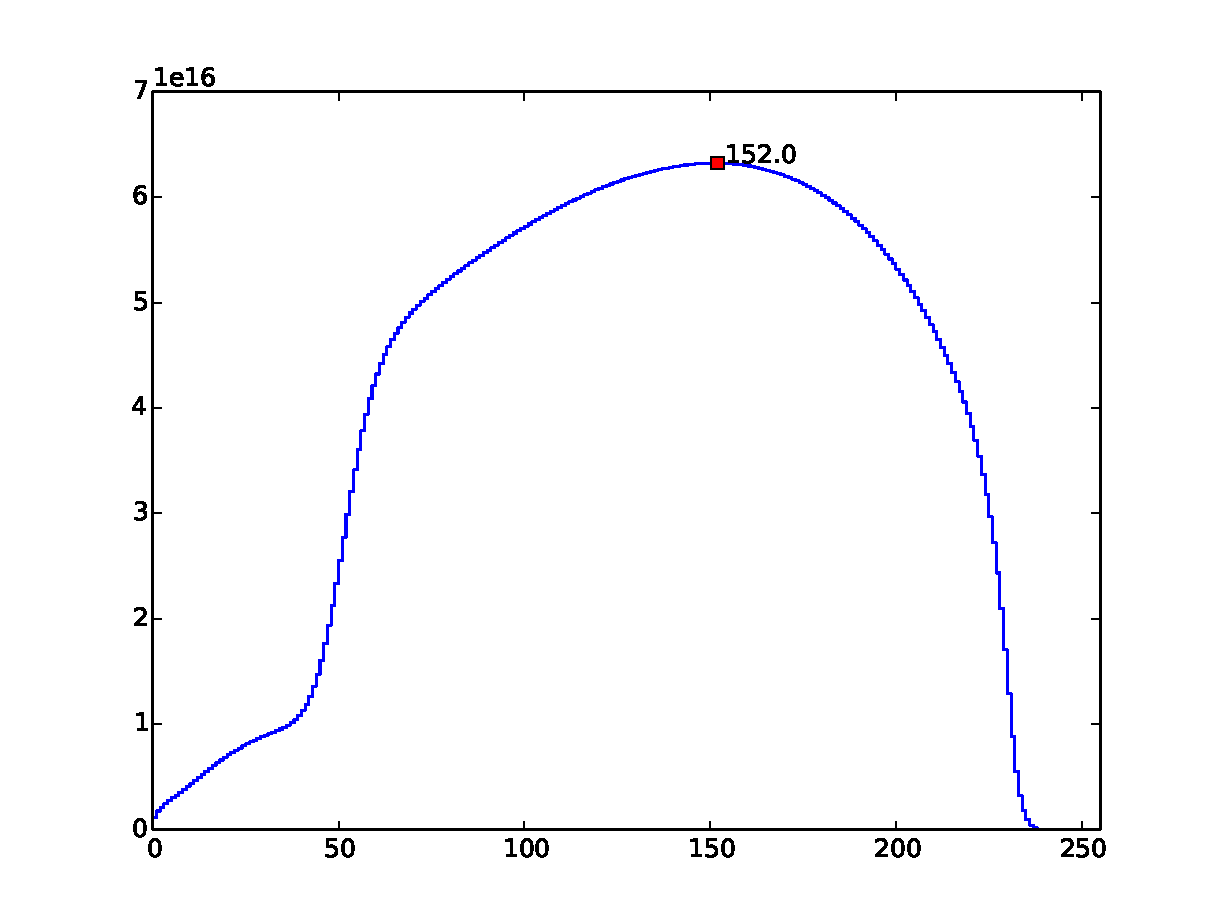
\includegraphics[width=0.5\linewidth]{./figure/interclass_variances}
\caption{Finding the maximum interclass variance}
\label{fig:interclass_variances}
\end{figure}

Otsu's method uses an exhaustive search to find the optimal solution.
As shown in Figure \ref{fig:interclass_variances}, when all the inter-class variances are obtained, select the maximum as the threshold.

\subsection{Implementation}

The functions are written in \emph{binarization.py}.

\begin{itemize}
\item \textbf{ otsu(hist, total) } reads the histogram and total number of the pixels, then returns the threshold.
\item \textbf{ binarize(img\_data, threshold, scale\_value=1) } converts the image data array into binary data array by threshold.
The binarize method can be viewed as converting the image to an 1-bit image with only 0 and 1.
The scale\_value can scale the value 1 to support higher bit image.
For 8-bit image, it becomes 255.
\end{itemize}

\subsection{Results}

%\subsubsection{0397.pgm}

The results of testing \emph{0397.pgm} are illustrated in Figure \ref{fig:binary:01}.

\begin{figure}[h]
\centering
\subfigure[Origin]{
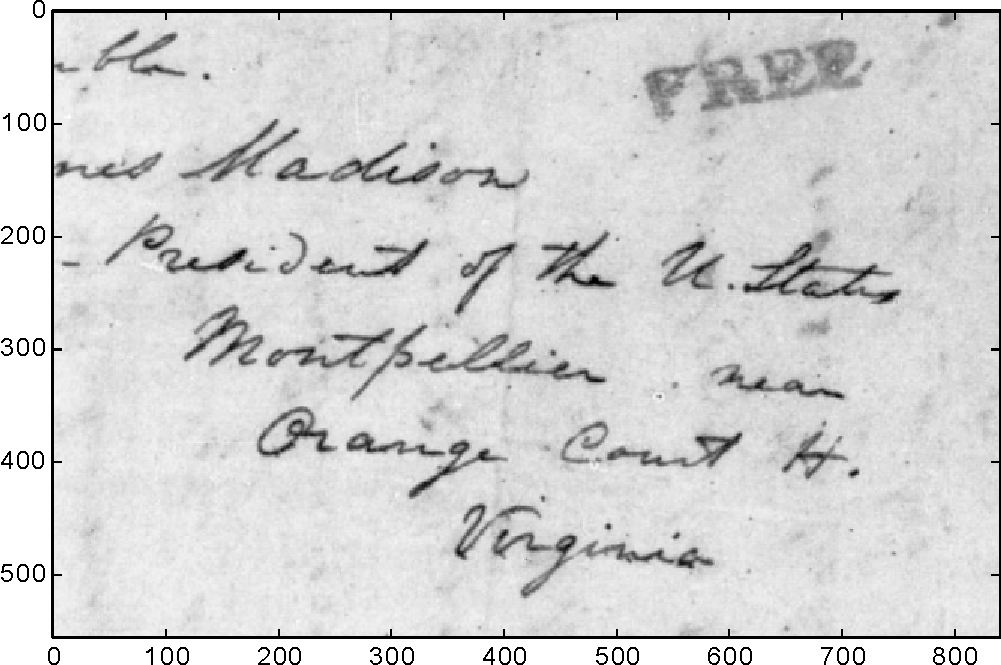
\includegraphics[width=.45\textwidth]{./figure/0397_pgm_origin}
\label{fig:binary:01:origin} }
\subfigure[Binary]{
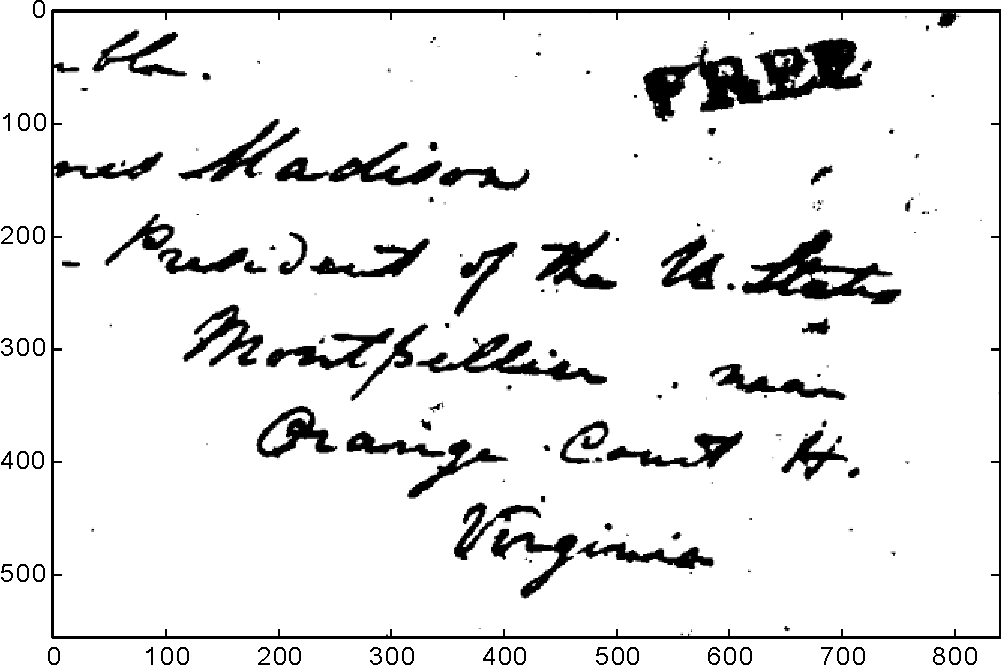
\includegraphics[width=.45\textwidth]{./figure/0397_pgm_binary}
\label{fig:binary:01:binary} }
\caption{Binarization of \emph{0397.pgm} using Otsu's method.}\label{fig:binary:01}
\end{figure}

\emph{020206\_131612\_bp001\_folio\_094\_k639\_1837.ppm} is also tested to show a case that the binarization works not very well.
The result is given in Figure \ref{fig:binary:02}.

\begin{figure}[h]
\centering
\subfigure[Origin]{
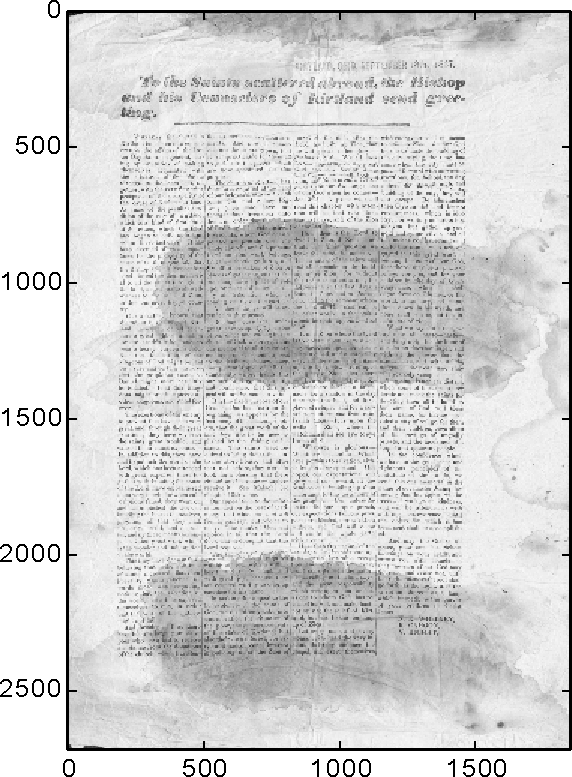
\includegraphics[width=.45\textwidth]{./figure/020206_131612_bp001_folio_094_k639_1837_ppm_origin}
\label{fig:binary:02:origin} }
\subfigure[Binary]{
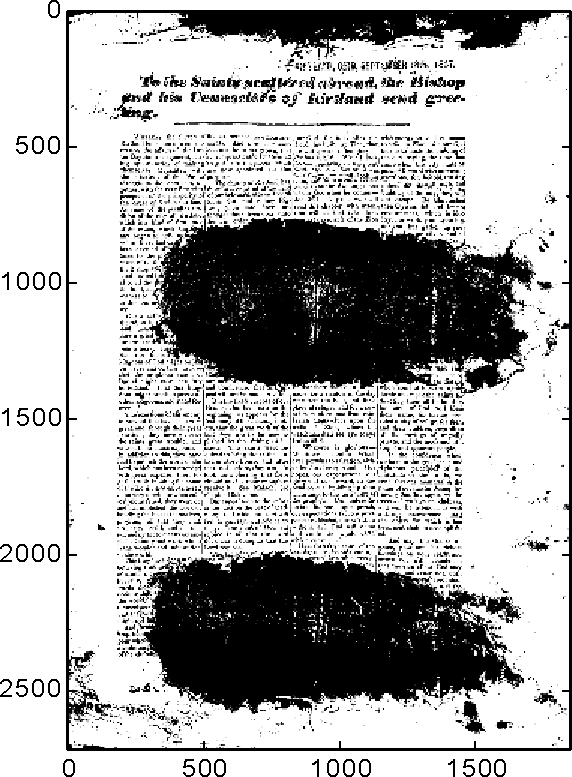
\includegraphics[width=.45\textwidth]{./figure/020206_131612_bp001_folio_094_k639_1837_ppm_binary}
\label{fig:binary:02:binary} }
\caption{Binarization of \emph{020206\_131612\_bp001\_folio\_094\_k639\_1837.ppm}  using Otsu's method.}\label{fig:binary:02}
\end{figure}

%\subsubsection{Other test files}

In order to check the correctness of the implementation, I compared the results from my implementation with the results from modules provided by open cv.
They are given in Table 1.1. %\ref{tab:title}.
When the thresholds are the same, the generated binary images should be consistent as well.
It is shown in Table 1.1 that the results are consistent.

\begin{table}[h]
\label{tab:binary_comp}
\caption {Comparison on the results of \textbf{threshold} obtained from different implementations of Otsu's method.}
\begin{center}
\begin{tabular}{ | l | l | l | }
\hline
Test file & Threshold (My code) & Threshold (Open CV)  \\ \hline
\emph{0397.pgm}                                          & 134 & 134 \\ \hline
\emph{020206\_131612\_bp001\_folio\_094\_k639\_1837.ppm} & 182 & 182 \\ \hline
\emph{Declaration\_Pg1of1\_AC\_crop.pgm}                 & 186 & 186 \\ \hline
\emph{Scan\_half\_crop\_norm\_009\_small.pgm}            & 134 & 134 \\ \hline
\emph{seq-4\_small.pgm}                                  & 152 & 152 \\ \hline
\end{tabular}
\end{center}
\end{table}

\subsection{Conclusion}

Otsu's method finds a threshold to separate the gray-scale pixels into two classes, which minimizes the intra-class variance.
The two classes are usually viewed as foreground and background.
When gray-scale values of the foreground pixels have significant difference with the gray-scale values of the background, Otsu's method shows good performance.
Figure \ref{fig:binary:01} is such an example.
The foreground pixels can be extracted well.
However, there are a lot of reasons that make the difference not significant, which can be caused by the light condition, stain and etc.
In these cases, the performance might not be ideal, as much information would be lost.
Figure \ref{fig:binary:02} gives an example like these.
In these cases, we could possibly cluster the background into several subregions.
Doing Otsu's method separately in each subregion might bring better results.

\section{Morphology}

The morphological operations use a box filter to count the number of ON pixels inside a range defined by the box filter.
For a binary image that is represented by 0 and 1, either pixel of 0 or pixel of 1 can be defined as ON pixel. 
In this lab, I choose pixel of 0 (BLACK pixel) as ON pixel.
Because the foreground objects are mostly black in the test files.

The \textbf{dilate} operation requires all the neighbor pixels in the box filter range are all ON so that the pixel can be set as ON, 
while the \textbf{erode} operation requires only one ON pixel in the box filter range.
The \texbtf{open} and \textbf{close} operations are combinations of the \textbf{dilate} and \textbf{erode} operations.
The \textbf{open} operation means doing \textbf{dilate} firstly and then \textbf{erode}.
The \textbf{close} operation follows a reversed sequence.

\subsection{Implementation}

The functions are written in \emph{morphology.py}.

\begin{itemize}
\item \textbf{ countNum( img\_data, maskSize ) } counts the number of ON pixels in the neighboring of each pixels. 
Because the mask cannot be completely applied in the corners, the mask data size might be different for different pixel.
Thus, an array of mask data size for each pixel is returned as well.
\item \textbf{ dataThreshold( data, threshold, ratio=1.0 ) } determines whether the number of ON pixels can surpass the threshold defined.
Ratio is added to support \textbf{majority} operation.
\end{itemize}

There is also a class \emph{MorphologicalFiltering}.
It stores the \emph{maskSizeData} used for operations \textbf{dilate}, \textbf{erode}, \textbf{open} and \textbf{close}.

\subsection{Results}

%\subsubsection{Letter J}


\begin{figure}
\centering
\subfigure[Binary]{
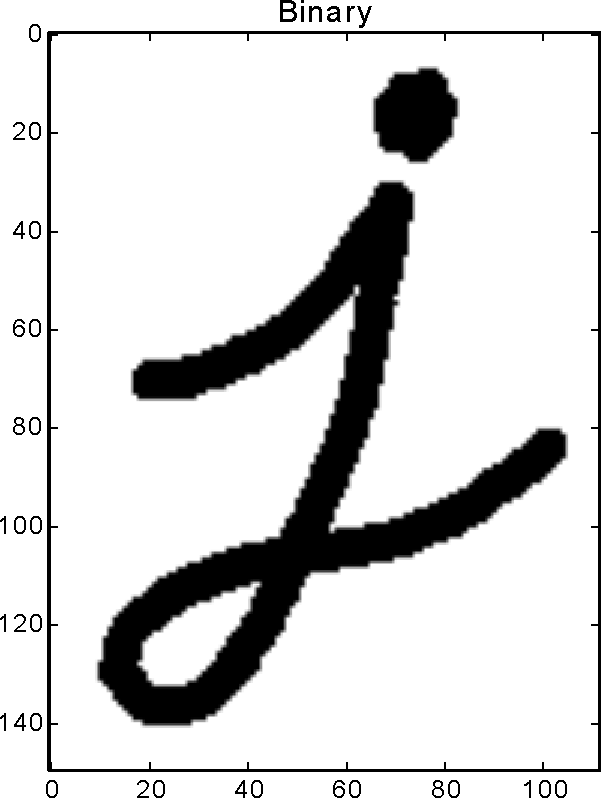
\includegraphics[width=.18\textwidth]{./figure/J_binary}
\label{fig:j_binary} }
\subfigure[Dilate]{
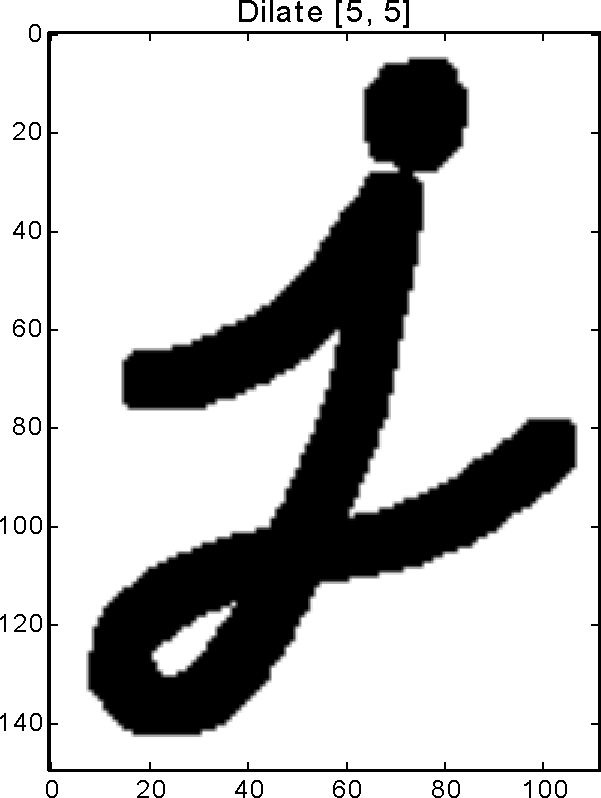
\includegraphics[width=.18\textwidth]{./figure/J_dilate}
\label{fig:j_dilate} }
\subfigure[Erode]{
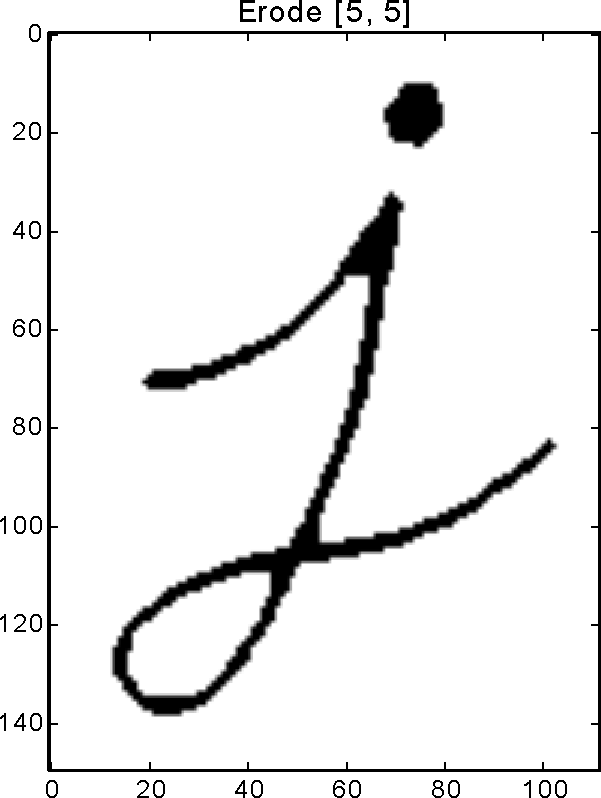
\includegraphics[width=.18\textwidth]{./figure/J_erode}
\label{fig:j_erode} }
\subfigure[Open]{
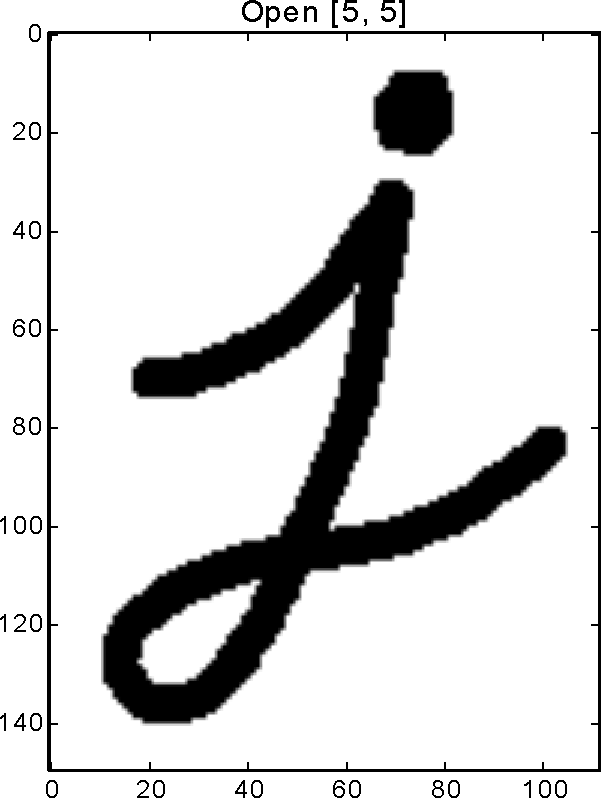
\includegraphics[width=.18\textwidth]{./figure/J_open}
\label{fig:j_open} }
\subfigure[Close]{
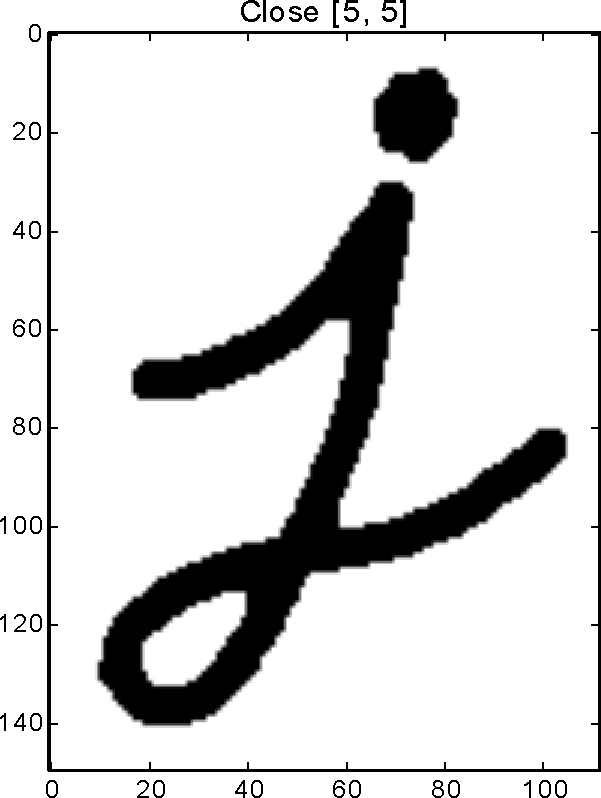
\includegraphics[width=.18\textwidth]{./figure/J_close}
\label{fig:j_close} }
\caption{Morphology operations on Letter J [$ 5 \times 5 $].}
\label{fig:j_letter}
\end{figure}

I use the image of Letter J to visually verify the correctness of my implementation, which is provided in Figure \ref{fig:j_letter}.
I also test different size of box filters on the \emph{0397.pgm} with \textbf{open} and \textbf{close} operations.
The effect of changing the size of box filter is illustrated in Figure \ref{fig:morph:01}.

%\subsubsection{0397.pgm}

\begin{figure}[h]
\centering
\subfigure[Open $ 5 \times 5 $]{
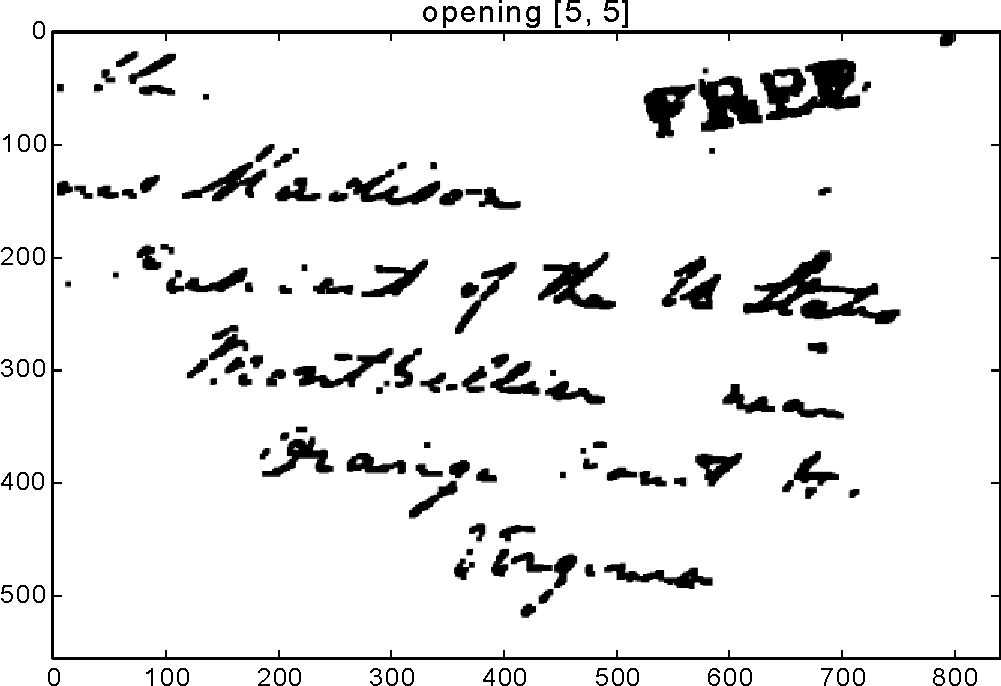
\includegraphics[width=.31\textwidth]{./figure/0397_pgm_open_5}
\label{fig:morph:01:open:5} }
\subfigure[Open $ 7 \times 7 $]{
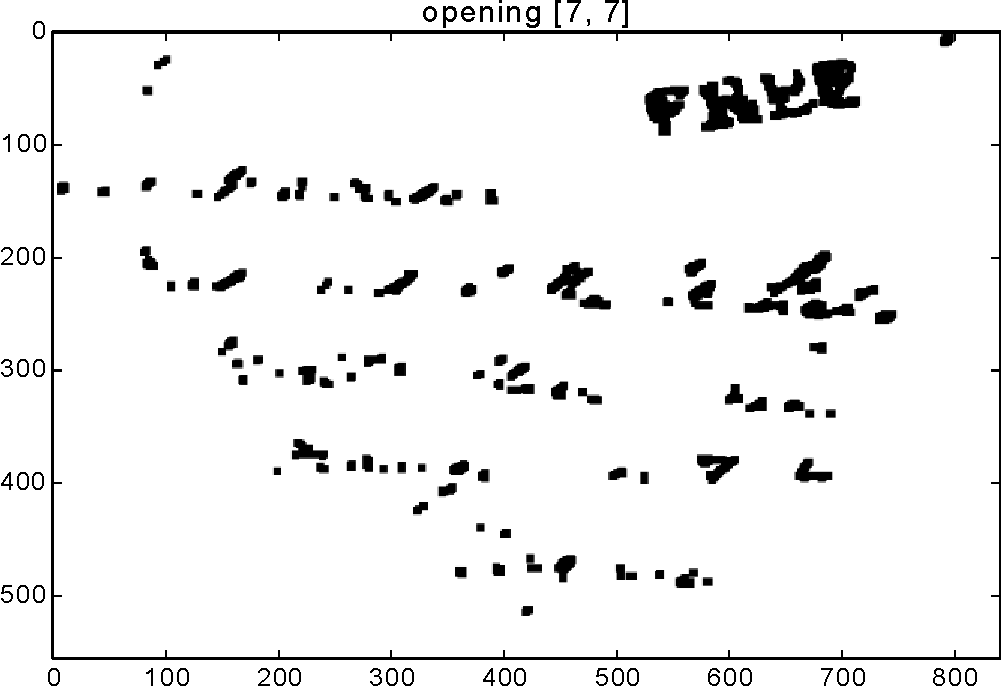
\includegraphics[width=.31\textwidth]{./figure/0397_pgm_open_7}
\label{fig:morph:01:open:7} }
\subfigure[Open $ 9 \times 9 $]{
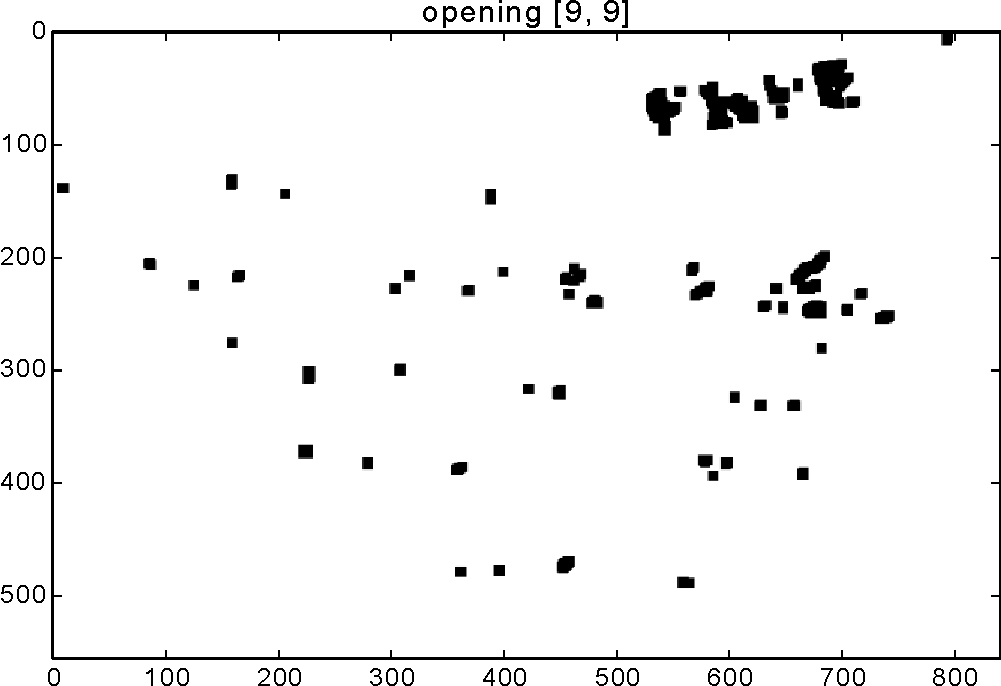
\includegraphics[width=.31\textwidth]{./figure/0397_pgm_open_9}
\label{fig:morph:01:open:9} }
\\
\subfigure[Colse $ 5 \times 5 $]{
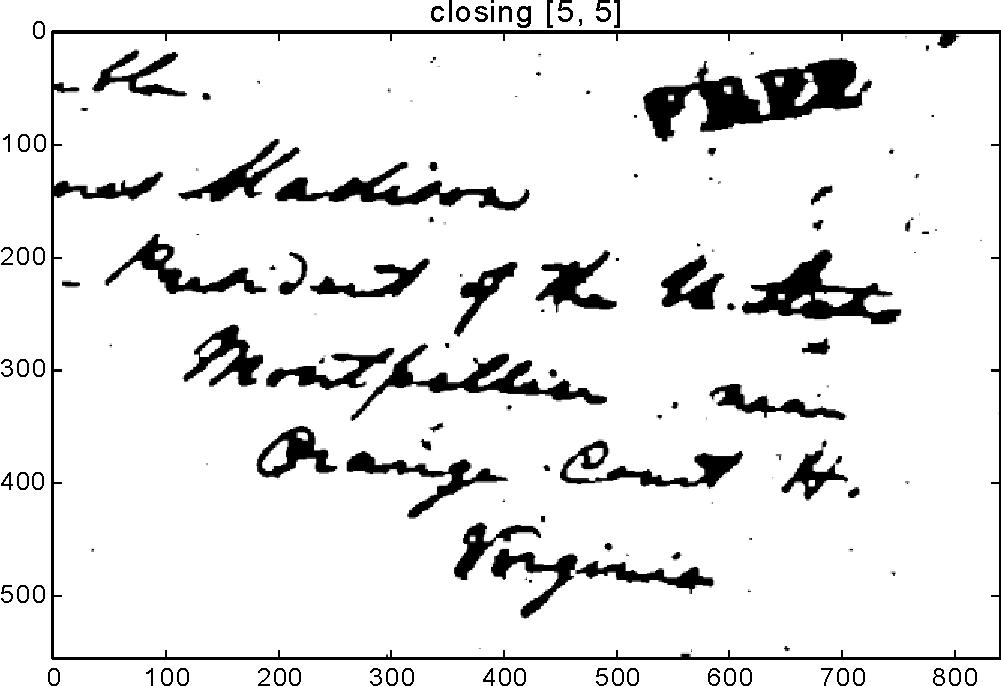
\includegraphics[width=.31\textwidth]{./figure/0397_pgm_close_5}
\label{fig:morph:01:close:5} }
\subfigure[Colse $ 5 \times 5 $]{
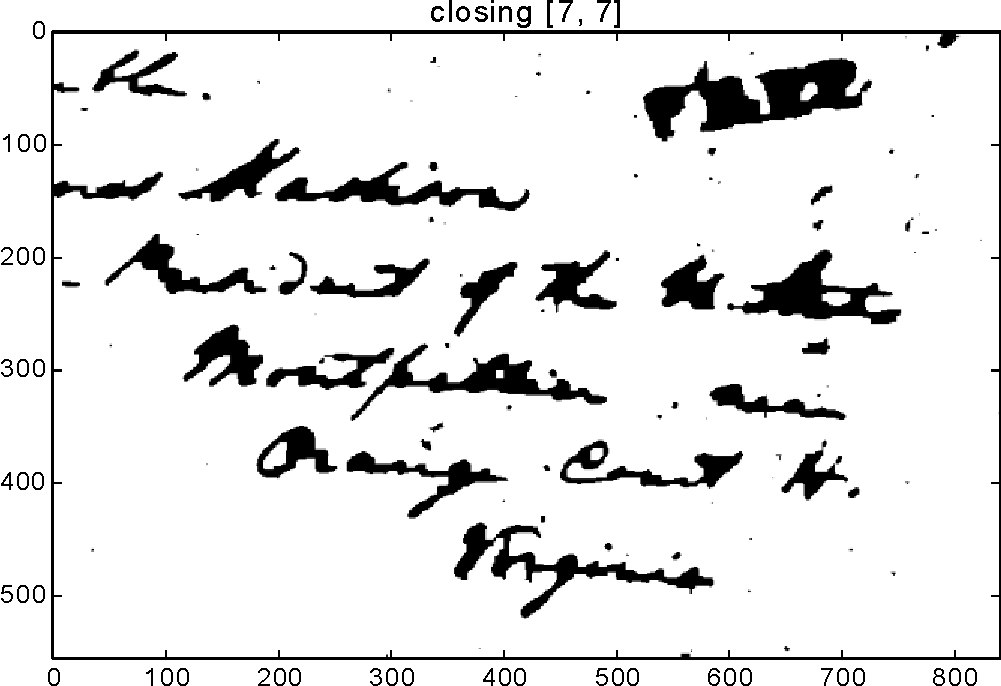
\includegraphics[width=.31\textwidth]{./figure/0397_pgm_close_7}
\label{fig:morph:01:close:7} }
\subfigure[Colse $ 9 \times 9 $]{
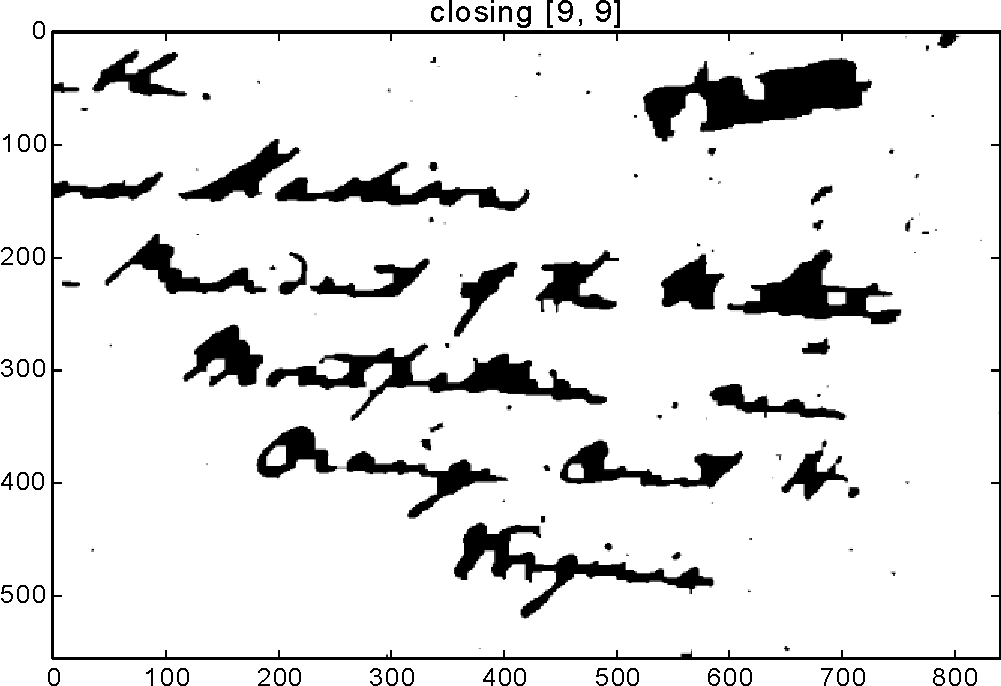
\includegraphics[width=.31\textwidth]{./figure/0397_pgm_close_9}
\label{fig:morph:01:close:9} }
\caption{Open and close operations on \emph{0397.pgm} [$ 5 \times 5 $].}
\label{fig:morph:01}
\end{figure}

%\subsubsection{Other test files}

In order to verify the correctness of the generated results, I use $ mean( abs( img - img\_ref ) ) $ to compare the data arrays from my implementation with the data arrays from open cv.
$ img $ is the data array from my implementation and $ img\_ref $ is the data array from open cv.
Because open cv use pixel of 1 as ON pixel, which is the reverse of my way.
In comparison, I compare my ``dilate'' to with the ``erode'' in open cv, and my ``erode'' with ``dilate'' in open cv.
Similarly, because ``open'' and ``close'' are reversed operation, I compare them in the same way.
The results are given in Table 2.1.
It is noticeable the results match for most of the files.
The difference is very small for the unmatch one, \emph{020206\_131612\_bp001\_folio\_094\_k639\_1837.ppm}.
Because I convert 1 to 255 before comapring.
Mean difference less than 1, relative to 255, means only several pixels are different.

\begin{table}
\label{tab:morphology_comp}
\caption {Comparison on the results of \textbf{threshold} obtained from different implementations of Morphological filter.}
\begin{center}
\begin{tabular}{ | l | l | l | l | l | }
\hline
Test file & Dilate & Erode & Open & Close  \\ \hline
Letter J                                                 & 0.0    & 0.0    & 0.0    & 0.0    \\ \hline
\emph{0397.pgm}                                          & 0.0    & 0.0    & 0.0    & 0.0    \\ \hline
\emph{020206\_131612\_bp001\_folio\_094\_k639\_1837.ppm} & 0.6943 & 1.1146 & 0.7899 & 0.6237 \\ \hline
\emph{Declaration\_Pg1of1\_AC\_crop.pgm}                 & 0.0    & 0.0    & 0.0    & 0.0    \\ \hline
\emph{Scan\_half\_crop\_norm\_009\_small.pgm}            & 0.0    & 0.0    & 0.0    & 0.0    \\ \hline
\emph{seq-4\_small.pgm}                                  & 0.0    & 0.0    & 0.0    & 0.0    \\ \hline
\end{tabular}
\end{center}
\end{table}

\begin{figure}[h]
\centering
\subfigure[Origin]{
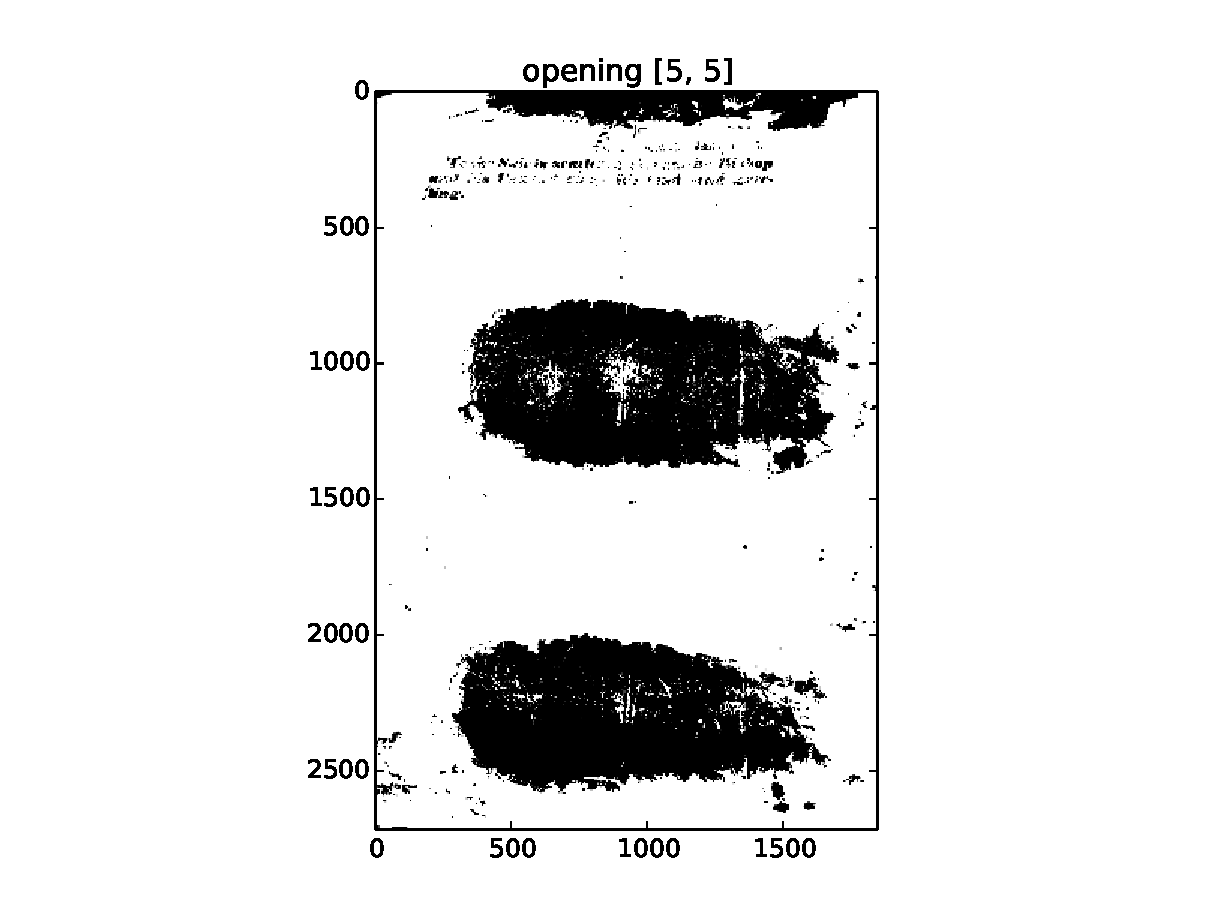
\includegraphics[width=.45\textwidth]{./figure/020206_131612_bp001_folio_094_k639_1837_ppm_open}
\label{fig:morph:02:open} }
\subfigure[Binary]{
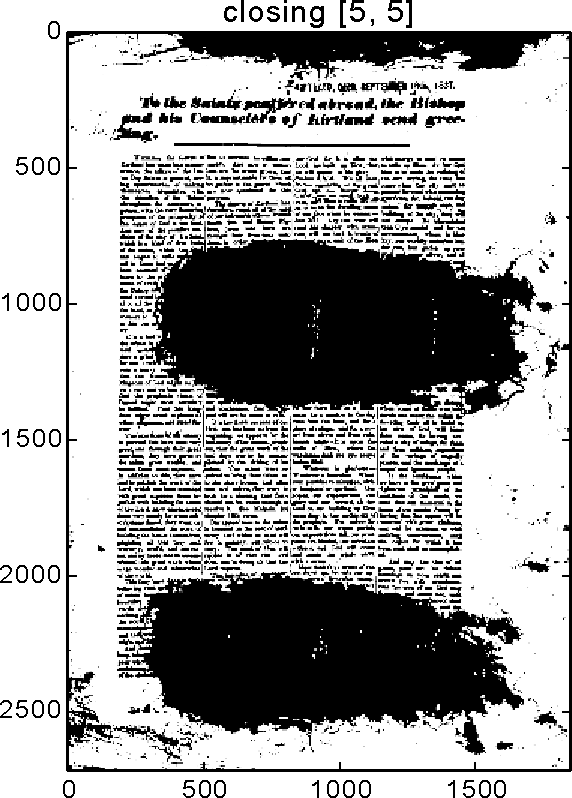
\includegraphics[width=.45\textwidth]{./figure/020206_131612_bp001_folio_094_k639_1837_ppm_close}
\label{fig:morph:02:close} }
\caption{Open and close operations of \emph{020206\_131612\_bp001\_folio\_094\_k639\_1837.ppm}.}
\label{fig:morph:02}
\end{figure}

\subsection{Conclusion}

I choose the black pixel as the ON pixel.
Because the foreground objects are black and I would like to show the morphological operations on the foreground objects.
The effects of the \textbf{dilate} and the \textbf{erode} are obvious in Figure \ref{fig:j_letter}.
\textbf{open} operation tends to remove small objects.
Because there is no small object, there is no significant effect.
\textbf{Close} tends to fill the ``holes'' in the objects or connect the objects are near enough.
We can see this in the \textbf{close} of Figure \ref{fig:j_close}.

The growth of the box filter size can influence the \textbf{open} significantly, as it is shown in Figure \ref{fig:morph:01}.
In Figure \ref{fig:morph:02}, \textbf{open} cleaned some noise but some useful information are also removed.
Because the size of each character is small relative to the box filter size.
\textbf{Close} is more likely to fill the ``holes'' inside the foreground objects when the box filter size is larger.
It is shown in Figure \ref{fig:morph:01}.

Selecting a good mask size, \textbf{open} can be used to denoise in an image with reasonable resolution.
Small objects will be removed as a result.
Similarly, \textbf{close} can be used to make the foreground objects more convex or become closed objects.
It can be viewed as denoise as well in some cases.
The weakness sometimes comes from the shape of the filter, if a square one is chose for the box filter.
For some particular shapes, a customized shape filter might have better performance.

\end{document}